\section{Introduction}
\label{sec:intro}

The exponential growth of digital image data has made it necessary to develop efficient systems for retrieving
relevant images from vast repositories. Image retrieval systems play a crucial role in various domains, including
medical imaging, multimedia content management, and e-commerce. One of the most notable applications of visual
search is Google Lens.

CBIR (Content-Based Image Retrieval) and TBIR (Text-Based Image Retrieval) are two approaches to retrieving images
from a database based on their content or associated textual information. This paper explores Content-Based Image
Retrieval.

Image retrieval systems need to be able to identify features of an image and generate descriptors.
These descriptors are then used to compare the features of different
images. Based on these comparisons, the image retrieval system ranks the images according to its similarity.
Figure \ref{fig:image_retrieval_flowchart} gives an overview of how a simple image retrieval system works.

\begin{figure}[htbp]
  \begin{center}
    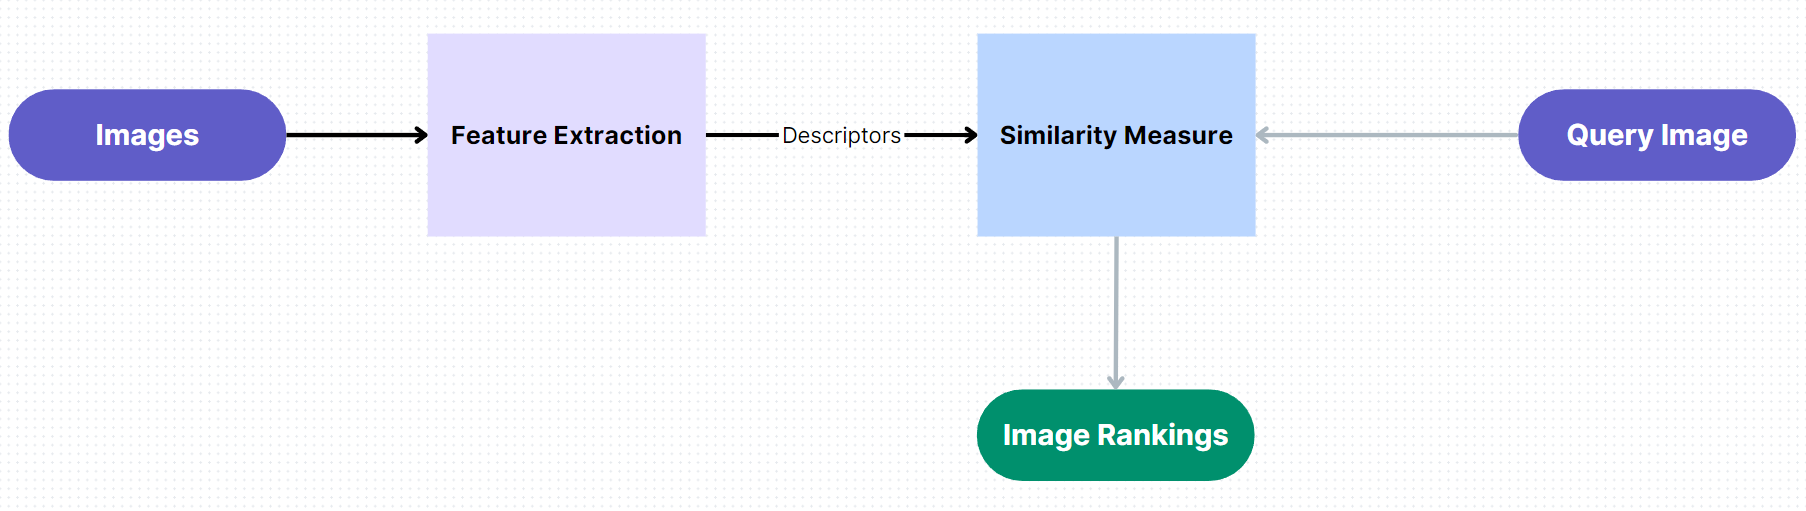
\includegraphics[width=0.75\textwidth]{./assets/image_retrieval_flowchart.png}
    \caption{Flowchart of a simple image retrieval system}
    \label{fig:image_retrieval_flowchart}
  \end{center}
\end{figure}
